\section{Darstellungsprobleme auf der Webseite}
Die Webseite der Wetterstation Arbon besteht neben der Homepage aus zwölf Unterseiten. Für uns wichtig sind all jene, die mit den Sensordaten, der Webcam, oder der Datebank in Verbindung stehen. (hervorgehoben in Abb.\ref{img:sitemap}). Im folgenden werden diese Seiten und deren Probleme genauer erläutert.

\begin{figure}[h!]
	\centering
	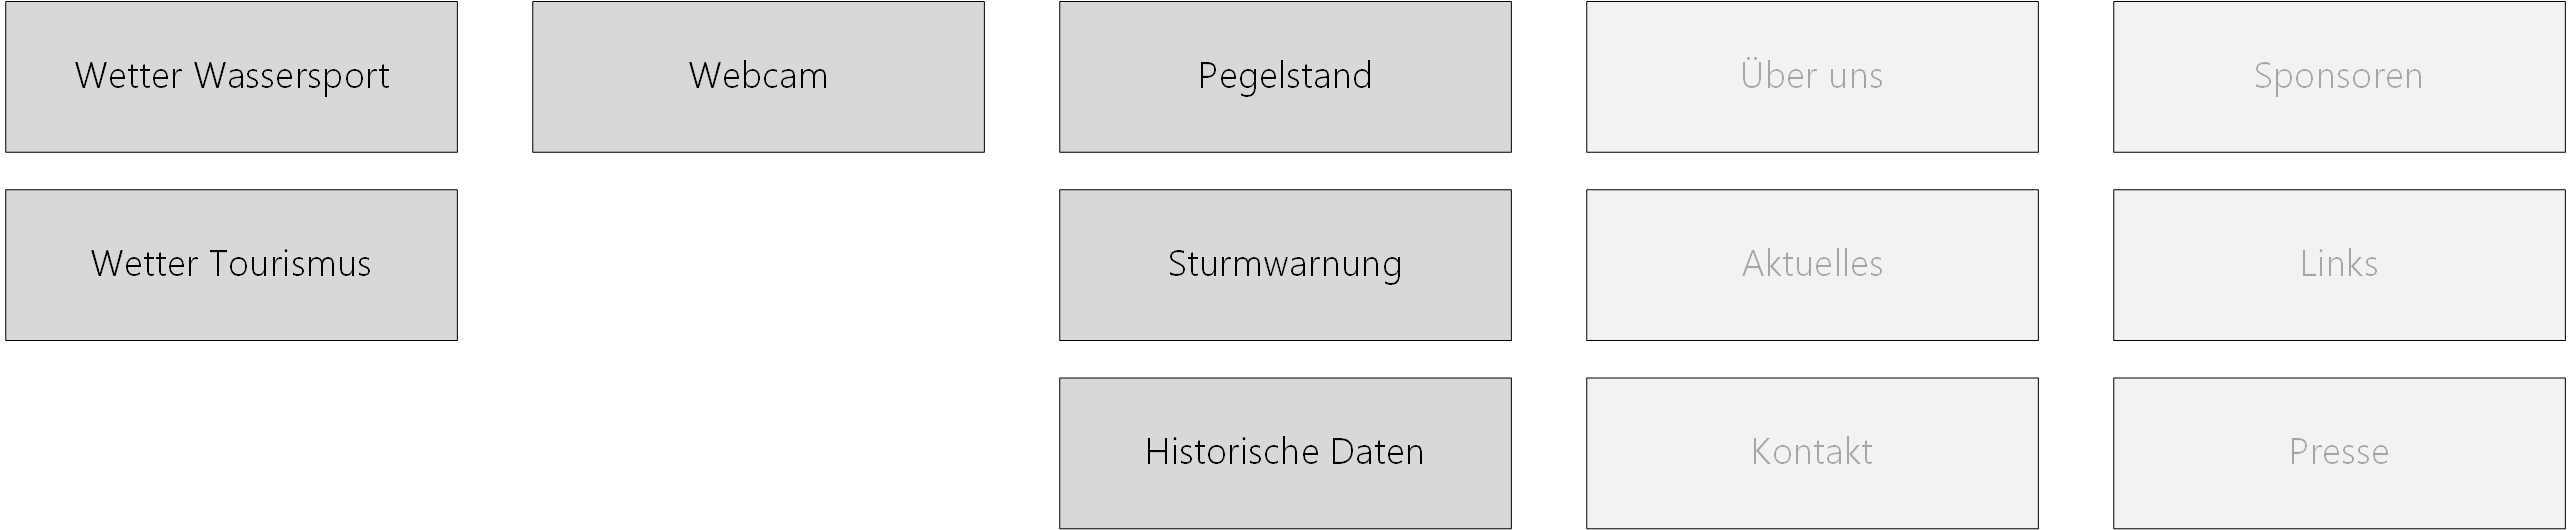
\includegraphics[width=0.9\linewidth]{img/sitemap}
	\caption{Sitemap der Webseite}
	\label{img:sitemap}
\end{figure}


\subsection{Adobe Flash: Workaround mit Nachteilen}

% ################################
% Problem Adobe Flash
% ################################
Um die Daten des Wettertransmitters auszulesen, wird Weather Display \footnote{ \url{http://www.weather-display.com/index.php }} verwendet. Dieses Programm liest die Daten des Wettertransmitters und stellt sie anderen Programmen zum Beispiel in Form eines Text-Files zur Verfügung. Weahter Display Live (WDL) \footnote{ \url{http://www.weather-display.de }} liest nun eben dieses Text-File und erstellt damit eine Adobe Flash Animations wie in Abb.\ref{img:responsive} dargestellt (gelb markiert).

Adobe Flash war eine einfache Möglichkeit animierte Grafiken auf Webseiten darzustellen und wurde praktisch von allen Browsern, nach Installation des Plug-ins, unterstützt. Diverse Sicherheitslücken und der Umstand, dass es sich um eine proprietäre d.h. closed-source Software handelte, führten dazu, dass Apple entschied Adobe Flash auf ihrem Mobile-Betiebsystem iOS nicht mehr zu unterstützen. \cite{Apple:ThoughtsOnFlash} 

Sämtliche Adobe Flash Animationen können somit nicht auf iPhone und iPad angezeigt werden. Da ein Grossteil der schweizer Bevölkerung jedoch genau diese Mobilgeräte verwendet, wurde für die Wetterstation folgender Workaround geschaffen: Der Browser prüft zuerst, ob das Gerät Adobe Flash unterstützt. Wenn ja wird die normale Applikation geladen, wenn nicht wird ein Printscreen der Applikaiton geladen (Code: \ref{lst:flash})

\begin{lstlisting}[caption={Adobe Flash workaround für iOS},label={lst:flash},language=html]
if (swfobject.hasFlashPlayerVersion("1")) {document.write('
<iframe src="https://www.wetter-arbon.ch/WDL/index.html"></iframe>');} 
else {document.write('
<img class="pageImage" src="https://www.wetter-arbon.ch/WDL/WDL.png" />');}
\end{lstlisting}

% Problem Workaround
Der Nachteil dieses Workarounds ist jedoch, dass die Anzeige weder dynamisch noch interaktiv ist. Um die aktuellen Werte zu erhalten muss die Seite jeweils neu geladen werden. Die interaktiven Elemente sind unbrauchbar d.h. die Änderung von Einheiten, Anzeige von Rekordwerten und weiteren Graphen ist nicht möglich.

\begin{figure}[h!]
	\centering
	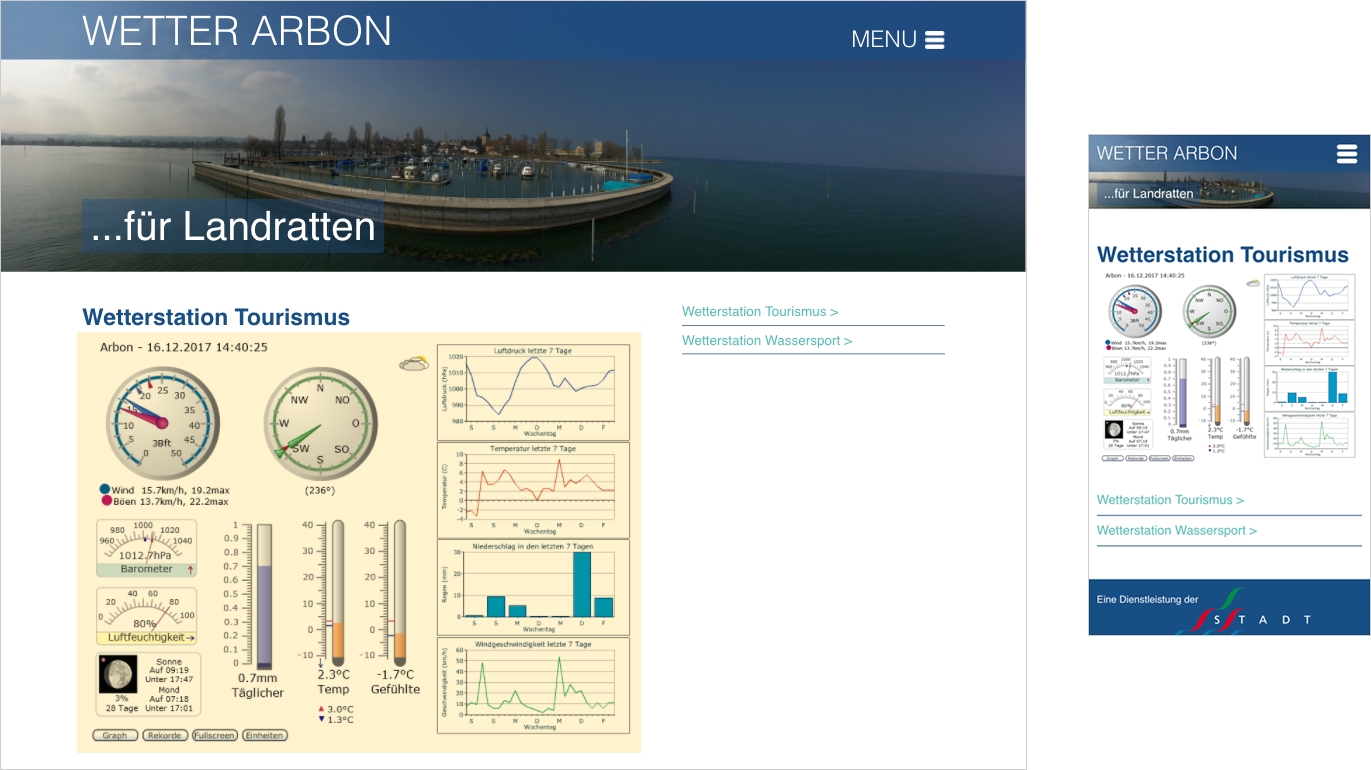
\includegraphics[width=1\linewidth]{img/responsive}
	\caption{Responsive Design; Problem Flash-Applikation}
	\label{img:responsive}
\end{figure}


% Lösung Flash
Mit dem aufkommen der Smartphones wurde Flash immer weiter verdrängt durch HTML5 und Javascript. Dadurch haben auch andere Hersteller von mobilen Geräten nachgezogen und auf Flash möglichst verzichtet. 

Der wichtigste Grund ist das Adobe ab 2020 Flash nicht mehr weiterentwickelt und keine Updates mehr herausgeben wird. Dies aufgrund der oben genannten Tatsachen und das zur heutigen Zeit vielmals Flash umgangen wird und andere Lösungen gebraucht werden. Aufgrund von dies wird ab 2020 auch kein Browser mehr das Plugin zulassen und Seiten welche Flashinhalte benutzen sind nicht mehr Vollständig verfügbar. Somit ist auch die Wetter-Arbon Seite von dieser Tatsache betroffen. \cite{Adobe:FlashTheFutureofInteractiveContent}\\


% ################################
% Problem Responsive Design
% ################################
\subsection{Wetterdaten ohne Responsive Design}
Die Webseite der Wetterstation ist mit dem Content-Management-System (CMS) \textit{Openfile64Light} der Firma Screenbox erstellt. Dieses unterstütz grundsätzlich responsive Design. Eigene Änderungen oder dynamische Inhalte, werden in openfile64Light als sogenannte Applikationen behandelt und in die Seite eingebettet. Unterstützt die eingebettete Applikation kein responsive Design, so wird dieser Teil einfach linear skaliert. Dies führt dazu, dass die Anzeige der Wetterstationsdaten auf einem Mobilgerät kaum mehr lesbar sind. (Abbildung \ref{img:responsive})





% ################################
% Problem Graphen
% ################################
\subsection{Verwirrende Graphen}
\Diskussionspunkt{Einführung zum Thema Graphen hinzufügen; wo werden sie dargestellt, was ist das Ziel}


% Windgeschwindigkeit
\subsubsection*{Automatische y-Skalierung von Graphen}
Die Graphen, bspw. der Windanzeige mit ihrer Richtung sowie die Stärke, sind schwer lesbar, da die Skalierung des Graphen automatisch die, je nach Windstärke, wechselt.

\Diskussionspunkt{Genauere Erklärung mit Bezug auf das Bild hinzufügen}

\begin{figure}[h!]
	\centering
	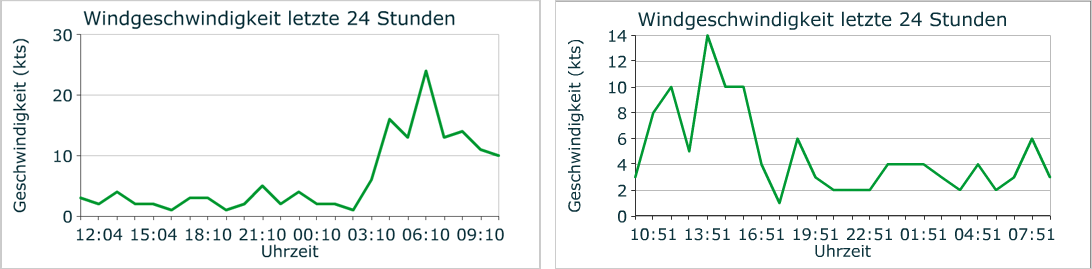
\includegraphics[width=1\linewidth]{img/wind-geschw}
	\caption{Anzeige der Windgeschwindigkeit mit variabler y-Skalierung}
	\label{img:wind-geschw}
\end{figure}



% Windrichtung
\subsubsection*{Windrichtung}

\Diskussionspunkt{Bild der Windrichtungsproblematik}

\Diskussionspunkt{Erklärung der Problematik}


% ################################
% Problem Sturmwarnung
% ################################
\subsection{Unsichere Sturmwarnung mit Öffnungszeiten}
Die Seite mir der Sturmwarnung, siehe \ref{img:sturm}, wurde anfangs November umgestellt aus Sicherheitsgründen, welche in der Problemanalyse erläutert werden. Zum jetzigen Zeitpunkt wird nur noch ein Link zur Verfügung gestellt um auf die kantonale Sturmwarnseite zu kommen. Die Daten dieser Seite werden mit dem deutschen Wetterdienst in Stuttgart sowie Meteo Schweiz erstellt und dienen auf der Webseite nur als Information. Zu beachten ist hierbei, dass die Sturmwarnungen Bürozeiten haben. D.h. konkret vom 1. April bis 31 Oktober zwischen 6 und 22 Uhr und vom 1. November bis 31. März zwischen 7 und 20 Uhr. Der deutsche Wetterdienst und Meteo Schweiz unterscheiden zwei verschiedene Kategorien. Zum einen starke Windböen zwischen 25 und 33 Knoten, dies wird 40 Blitze pro Minute an den Leuchten signalisiert. Zum anderen Sturmböen von 34 und mehr Knoten, welche mit 90 Blitze pro Minute signalisiert werden. Zusätzlich zu den beiden Kategorien wird der Bodensee in 3 verschiedene Zonen unterteilt, West, Mitte und Ost, wobei Arbon in zur Zone Ost gehört. Wie schon erklärt ist das Problem hierbei der HTTP Standard, viele der Webbrowser stellen die Unterstützung dieses Standards langsam aber sicher ein und werden dann nur noch HTTPS unterstützen\cite{Mozilla:DeprecatingNon-SecureHTTP}. Deswegen ist die Sturmwarnung nur über einen Link aufrufbar. 


\begin{figure}[h!]
	\centering
	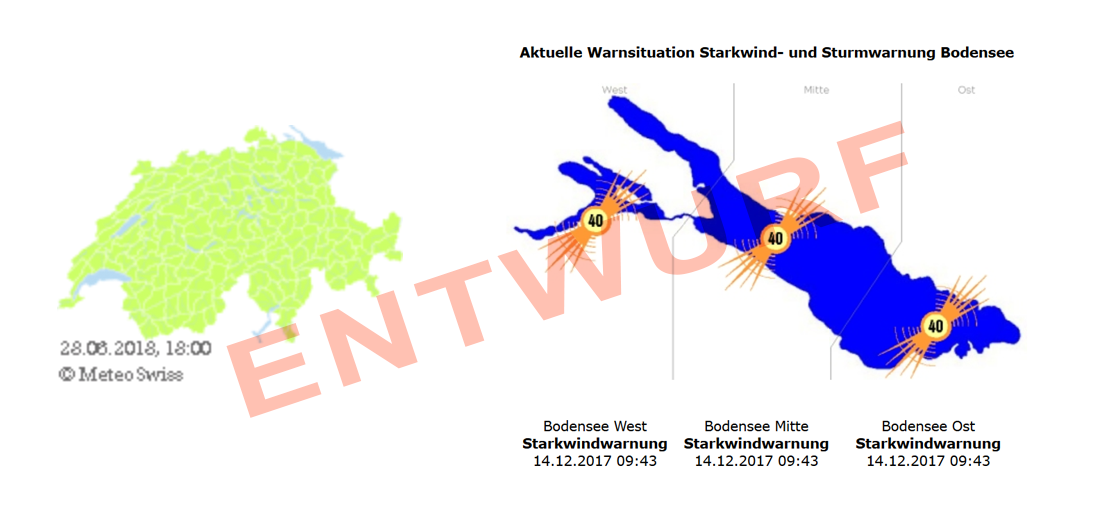
\includegraphics[width=1\linewidth]{img/sturm}
	\caption{Sturmwarnung vom Kanton Thurgau}
	\label{img:sturm}
\end{figure}




\Diskussionspunkt{Die folgenden Aussagen bitte beim jeweiligen Kapitel hinzufügen: }
Das Problem der Webseite und vorallem der verschiedenen Applikationen ist, dass viele Geräte Flash nicht mehr oder in naher Zukunft nicht mehr unterstützen. Zusätzlich ist die Lösung mit dem Screenshot der aktuellen Verhältnisse auch keine optimale Lösung. Auch sind die Schreibfehler, welche entdeckt wurden bei näherer Betrachtung auch nicht Vorteilhaft. Weiter ist die Wetterapplikation nicht nach dem Prinzip responsive Design aufgebaut, welches in der heutigen Zeit ein wichtiger Bestandteil einer Webseite ist. Zusätzlich zum Flash, von der Gebrauch gemacht wird sind die Anzeigen auf der Touristik bzw. Wassersport Seite unschön. 

Um die Webseite auf den neusten Stand der Technik zu bringen sollten folgende Änderungen durchgeführt werden.Die Flash-Software wird ausgemustert und die Applikation wird auf HTML5 und Javascript umgestellt. Die Webseite soll zudem im responsive Design entwickelt werden, damit auch auf mobilen Geräten die aktuelle Wetterlage sichtbar ist. Die dynamischen, sowie auch die teilweise statischen Anzeigen, werden wo möglich mithilfe der Javascript Bibliothek D3.js oder Google Charts erstellt, hiermit lassen sich ansehnliche und moderne Grafiken erstellen. Die Grafiken, sollten so gestaltet sein das auch Sehbehinderte Personen erkennen wie das Wetter momentan ist. Das heisst beispielsweise, dass die Farben auch für Farbenblinde unterscheidbar sein sollten oder blinde Personen anhand eines Vorleseprogramms erkennen wie das Wetter ist. Ein weiterer Punkt ist die Auswahl der Einheiten, diese sollen nach dem ersten Besuch gespeichert bleiben beim Client mithilfe von Webstorage.
